% !TEX root = sum1.tex

\section{Results}
We carried out several experiments, including analyzing the performances of different policies, evaluating the impact of implementing social distancing.


\subsection{Performances of Different Policies}
In this section, we compare the performance of five dynamic seat assignment policies to the optimal value, which can be obtained by solving the deterministic model after observing all arrivals. The policies under examination are the stochastic planning policy, DP Base-heuristic, bid-price control, booking limit control and FCFS policy. 


\subsubsection*{Bid-price Control}
Bid-price control is a classical approach discussed extensively in the literature on network revenue management. It involves setting bid prices for different group types, which determine the eligibility of groups to take the seats. Bid-prices refer to the opportunity costs of taking one seat. As usual, we estimate the bid price of a seat by the shadow price of the capacity constraint corresponding to some row. In this section, we will demonstrate the implementation of the bid-price control policy. 

The dual of LP relaxation of problem \eqref{deter_upper} is:

\begin{equation}\label{bid-price_dual}
  \begin{aligned}
  \min \quad & \sum_{i=1}^{M} d_i z_i + \sum_{j= 1}^{N} L_j \beta_{j} \\
  \text {s.t.} \quad & z_{i} + \beta_j n_i \geq (n_i-\delta), \quad i \in \mathcal{M}, j \in \mathcal{N} \\
  & z_{i} \geq 0, i \in \mathcal{M}, \beta_{j} \geq 0, j \in \mathcal{N}.
  \end{aligned}
\end{equation}

In \eqref{bid-price_dual}, $\beta_{j}$ can be interpreted as the bid-price for a seat in row $j$. A request is only accepted if the revenue it generates is above the sum of the bid prices of the seats it uses. Thus, if its revenue is more than its opportunity costs, i.e., $i -\beta_{j} n_i \geq 0$, we will accept the group type $i$. And choose $j^{*} = \arg \max_{j} \{i -\beta_{j} n_i\}$ as the row to allocate that group.


\begin{lem}\label{bid-price}
 The optimal solution to problem \eqref{bid-price_dual} is given by $z_1 ,\ldots, z_{\tilde{i}} =0$, $z_{i} = \frac{\delta(n_i-n_{\tilde{i}})}{n_{\tilde{i}}}$ for $i = \tilde{i}+1, \ldots, M$ and $\beta_j = \frac{n_{\tilde{i}} - \delta}{n_{\tilde{i}}}$ for all $j$.
\end{lem}

The bid-price decision can be expressed as $i - \beta_j n_i = i - \frac{n_{\tilde{i}} - \delta}{n_{\tilde{i}}} n_i = \frac{\delta (i - \tilde{i})}{n_{\tilde{i}}}$. When $i < \tilde{i}$, $i - \beta_j n_i < 0$. When $i \geq \tilde{i}$, $i - \beta_j n_i \geq 0$. This means that group type $i$ with $i$ greater than or equal to $\tilde{i}$ will be accepted if the capacity allows. However, it should be noted that $\beta_j$ does not vary with $j$, which means the bid-price control cannot determine the specific row to assign the group to. In practice, groups are often assigned arbitrarily based on availability when the capacity allows, which can result in a large number of empty seats.

The bid-price control policy based on the static model is stated below.

\begin{algorithm}[H]
  \caption{Bid-price Control Algorithm}\label{algo_bid}
  \For{$t =1, \ldots, T$}{
    {Observe group type $i$\;}
    {Solve the LP relaxation of problem \eqref{deter_upper} with $d_i^{t} = (T-t) \cdot p_i$ and $\mathbf{L}^{t}$\;
    Obtain $\tilde{i}$ such that the aggregate optimal solution is $x e_{\tilde{i}} + \sum_{i=\tilde{i}+1} ^{M} d_{i} e_{i}$\;}
    \eIf{$i \geq \tilde{i}$ and $\max_j{L_j} \geq n_i$}
    {Accept the group and assign the group to row $k$ such that $L_{k} \geq n_{i}$\;  
    $\mathbf{L}^{t+1} \gets \mathbf{L}^{t} - n_i \mathbf{e}_{k}$\;}
    {Reject the group\; $\mathbf{L}^{t+1} \gets \mathbf{L}^{t}$\;}}
\end{algorithm}


\subsubsection*{Booking Limit Control}

The booking limit control policy involves setting a maximum number of reservations that can be accepted for each group type. By controlling the booking limits, revenue managers can effectively manage demand and allocate inventory to maximize revenue.

In this policy, we replace the real demand by the expected one and solve the corresponding static problem using the expected demand. Then for every type of requests, we only allocate a fixed amount according to the static solution and reject all other exceeding requests. When we solve the linear relaxation of problem \eqref{deter_upper}, the aggregate optimal solution is the limits for each group type. Interestingly, the bid-price control policy is found to be equivalent to the booking limit control policy.

When we solve problem \eqref{deter_upper} directly, we can develop the booking limit control policy.

\begin{algorithm}[H]
  \caption{Booking limit Control Algorithm}\label{algo_booking}
  \For{$t =1, \ldots, T$}{
    {Observe group type $i$\;}
    {Solve problem \eqref{deter_upper} with $d_i^{t} = (T-t) \cdot p_i$ and $\mathbf{L}^{t}$\;
    Obtain the optimal solution, $x_{ij}^{*}$ and the aggregate optimal solution, $\mathbf{X}$\;}
    \eIf{$X_i > 0$}
    {Accept the group and assign the group to row $k$ such that $x_{ik} > 0$\;  
    $\mathbf{L}^{t+1} \gets \mathbf{L}^{t} - n_i \mathbf{e}_{k}$\;}
    {Reject the group\; $\mathbf{L}^{t+1} \gets \mathbf{L}^{t}$\;}}
\end{algorithm}


\subsubsection*{Dynamic Programming Base-heuristic}
To simplify the complexity of the original dynamic programming problem, we can consider a simplified version by relaxing all rows to a single row with the same total capacity, denoted as $L = \sum_{j=1}^{N} L_j$. With this simplification, we can make decisions for each group arrival based on the relaxed dynamic programming. By relaxing the rows to a single row, we aggregate the capacities of all individual rows into a single capacity value. This allows us to treat the seat assignment problem as a one-dimensional problem, reducing the computational complexity. Using the relaxed dynamic programming approach, we can determine the seat assignment decisions for each group arrival based on the simplified problem.


Let $u$ denote the decision, where $u^{t} = 1$ if we accept a request in period $t$, $u^{t} =0$ otherwise. Similar to the DP in section \ref{sec_dynamic_seat}, the DP with one row can be expressed as:

$$V^{t}(l) =  \max_{u^{t} \in \{0,1\}} \left\{ \sum_{i} p_i [V^{t+1}(l-n_i u^{t})+ i u^{t}] + p_0 V^{t+1}(l)\right\} $$
with the boundary conditions $V^{T+1}(l) =0, \forall l \geq 0$, $V^{t}(0) =0, \forall t$.

After accepting one group, assign it in some row arbitrarily when the capacity of the row allows.

\begin{algorithm}[H]
  \caption{Dynamic Programming Base-heuristic Algorithm}\label{algo_dp_heuris}
  Calculate $V^{t}(l)$, $\forall t =2, \ldots, T; \forall l = 1, \ldots, L$\;
  $l^{1} \gets L$\;
  \For{$t =1, \ldots, T$}{
    {Observe group type $i$\;}
    \eIf{$V^{t+1}(l^{t}) \leq V^{t+1}(l^{t}-n_i) + i$}
    {Accept the group and assign the group to an arbitrary row $k$ such that $L_{k} \geq n_i$\;  
    $L_{k}^{t+1} \gets L_{k}^{t} - n_i$, $l^{t+1} \gets l^{t} - n_i$\;}
    {Reject the group\;
    $L_{k}^{t+1} \gets L_{k}^{t}$, $l^{t+1} \gets l^{t}$\;}}
\end{algorithm}

\subsubsection*{First Come First Served (FCFS) Policy}
For dynamic seat assignment for each group arrival, the intuitive but trivial method will be on a first-come-first-served basis. Each accepted request will be assigned seats row by row. If the capacity of a row is insufficient to accommodate a request, we will allocate it to the next available row. If a subsequent request can fit exactly into the remaining capacity of a partially filled row, we will assign it to that row immediately. Then continue to process requests in this manner until all rows cannot accommodate any groups.

\begin{algorithm}[H]
  \caption{FCFS Policy Algorithm}\label{algo_fcfs}
  \For{$t =1, \ldots, T$}{
    {Observe group type $i$\;}
    \eIf{$\exists k$ such that $L_{k} \geq n_i$}
    {Accept the group and assign the group to row $k$\;  
    $L_{k} \gets L_{k} - n_i$\;}
    {Reject the group\;}}
\end{algorithm}

\subsubsection*{Numerical Results}
The seat layout consists of 10 rows, each with 21 seats (including one dummy seat as the social distance), and the group size can range up to 4 people. We conducted experiments over 60 to 100 periods to demonstrate the policies' performance under varying demand levels. We selected three probabilities to ensure that the expected number of people for each period is consistent. The table below displays the average of 200 instances for each number.

An arrival sequence during $T$ periods can be expressed as ${y_1, y_2, \ldots, y_T}$. Let $N_i = \sum_{t} I(y_t = i)$, i.e., the count number of times group type $i$ arrives during $T$ periods. Then the scenarios, $(N_1, \ldots, N_M)$, follow a multinomial distribution, 
$$
p\left(N_1, \ldots, N_M \mid \mathbf{p}\right)=\frac{T !}{N_{1} !, \ldots, N_{M} !} \prod_{i=1}^M p_i^{N_i}, T=\sum_{i=1}^M N_i.
$$

It is clear that the number of different sequences is $M^T$. The number of different scenarios is
$O(T^{M-1})$ which can be obtained by the following DP. The number of scenarios is too large to enumerate all possible cases. Thus, we choose to sample some sequences from the multinomial distribution.


\begin{table}[ht]
  \centering
  \caption{Performances of Different Policies}
  \begin{tabular}{|l|l|l|l|l|l|l|}
  \hline
   T & probabilities & DSA (\%) & DP1 (\%) & Bid-price (\%) & Booking (\%) & FCFS (\%) \\
  \hline
   60  & [0.25, 0.25, 0.25, 0.25]  & 99.12 & 98.42 & 98.38 & 96.74 & 98.17 \\
   70  &                           & 98.34 & 96.87 & 96.24 & 97.18 & 94.75 \\
   80  &                           & 98.61 & 95.69 & 96.02 & 98.00 & 93.18 \\
   90  &                           & 99.10 & 96.05 & 96.41 & 98.31 & 92.48 \\
   100 &                           & 99.58 & 95.09 & 96.88 & 98.70 & 92.54 \\
   \hline
   60  & [0.25, 0.35, 0.05, 0.35]  & 98.94 & 98.26 & 98.25 & 96.74 & 98.62 \\
   70  &                           & 98.05 & 96.62 & 96.06 & 96.90 & 93.96 \\
   80  &                           & 98.37 & 96.01 & 95.89 & 97.75 & 92.88 \\
   90  &                           & 99.01 & 96.77 & 96.62 & 98.42 & 92.46 \\
   100 &                           & 99.23 & 97.04 & 97.14 & 98.67 & 92.00 \\
  \hline
  60  & [0.15, 0.25, 0.55, 0.05]  & 99.14 & 98.72 & 98.74 & 96.61 & 98.07 \\
  70  &                           & 99.30 & 96.38 & 96.90 & 97.88 & 96.25 \\
  80  &                           & 99.59 & 97.75 & 97.87 & 98.55 & 95.81 \\
  90  &                           & 99.53 & 98.45 & 98.69 & 98.81 & 95.50 \\
  100 &                           & 99.47 & 98.62 & 98.94 & 98.90 & 95.25 \\
  \hline
  \end{tabular}
\end{table}

We can find that the stochastic planning policy are better than DP Base-heuristic and bid-price policy consistently, and FCFS policy works worst. As we mentioned previously, DP Base-heuristic and bid-price policy can only make the decision to accept or deny, cannot decide which row to assign the group to. FCFS accepts groups in sequential order until the capacity cannot accommodate more.


For the first three policies, their performance tends to initially drop and then increase as the number of periods increases. When the number of periods is small, the demand for capacity is relatively low, and the policies can achieve relatively optimal performance. However, as the number of periods increases, the policies may struggle to always obtain a perfect allocation plan, leading to a decrease in performance. Nevertheless, when the number of periods continue to become larger, these policies tend to accept larger groups, and as a result, narrow the gap with the optimal value, leading to an increase in performance.


\subsection{Impact of Implementing Social Distancing in DSA}
In this section, our focus is to analyze the influence of social distancing on the number of accepted individuals. Intuitively, when demand is small, we will accept all arrivals, thus there is no difference whether we implement the social distancing. What is interesting for us is when the difference occurs. Our primary objective is to determine the first time period at which, on average, the number of people accepted without social distancing is not less than the number accepted with social distancing plus one. This critical point, referred to as the gap point, is of interest to us. Additionally, we will examine the corresponding occupancy rate at this gap point. It should be noted that the difference at a specific time period may vary depending on the total number of periods considered. Therefore, when evaluating the difference at a particular time period, we assume that there are a total of such periods under consideration.


It is evident that as the demand increases, the effect of social distancing becomes more pronounced. We aim to determine the specific time period where the absence of social distancing results in a higher number of accepted individuals compared to when social distancing measures are in place. Additionally, we will calculate the corresponding occupancy rate during this period.

By analyzing and comparing the data, we can gain insights into the relation between demand, social distancing, the number of accepted individuals, and occupancy rates. This information is valuable for understanding the impact of social distancing policies on overall capacity utilization and making informed decisions regarding resource allocation and operational strategies.

\subsubsection{Estimation of Gap Point}
Based on our findings, we observed that the seat allocation derived from the optimal solution consistently satisfies the formation of either the largest pattern or the full pattern, regardless of different probability combinations. However, certain counterexamples arise when the requirements associated with specific probability combinations are unable to form a full pattern, resulting in gaps in the seating arrangement. The occurrence of these counterexamples is closely tied to the seat layout itself. The ratio of the number of largest patterns to the number of full patterns in the final seat allocation is influenced by the expected number of people in each period. We can leverage the expected number of people in each period to estimate the gap point when utilizing the DSA. This approach allows us to approximate the period at which the number of people accepted without social distancing surpasses the number accepted with social distancing, based on the performance characteristics observed in the DSA.

To find such a first period, we aim to find the maximum period such that we could assign all the groups during these periods into the seats, i.e., for each group type $i$, we have $\sum_{j} x_{ij} \geq d_i$, where $x_{ij}$ is the number of group type $i$ in row $j$. Meanwhile, we have the capacity constraint $\sum_{i} n_{i} x_{ij} \leq L_j$, thus, $\sum_{i} n_i d_i \leq \sum_{i} n_i \sum_{j} x_{ij} \leq \sum_{j} L_{j}$. Notice that $E(d_i) = p_i T$, we have $\sum_{i} n_i p_i T \leq \sum_{j} L_{j}$ by taking the expectation. Let $L = \sum_{j} L_{j}$, representing the total number of seats, $\gamma = \sum_{i} i p_i$, representing the average number of people who arrive in each period, we can obtain $T \leq \frac{L}{\gamma + \delta}$, then the upper bound of the expected maximum period is $T' = \frac{L}{\gamma + \delta}$.


Assuming that we accept all incoming groups within $T'$ periods, filling all the available seats, the corresponding occupancy rate at this period can be calculated as $\frac{\gamma T'}{(\gamma+ \delta)T' - N \delta} = \frac{\gamma}{\gamma +\delta} \frac{L}{L-N \delta}$. However, it is important to note that the actual maximum period will be smaller than $T{'}$ because it is impossible to accept groups to fill all seats exactly. To estimate the gap point when applying DSA, we can use $y_1 = c_1 \frac{L}{\gamma + \delta}$, where $c_1$ is a discount rate compared to the ideal assumption. Similarly, we can estimate the corresponding occupancy rate as $y_2 = c_2 \frac{\gamma}{\gamma +\delta} \frac{L}{L-N \delta}$, where $c_2$ is a discount rate for the occupancy rate compared to the ideal scenario.

We consider the scenario where the number of group types is limited to 4. In this case, the average number of people per period, denoted as $\gamma$, can be expressed as $\gamma = p_1 \cdot 1 + p_2 \cdot 2 + p_3 \cdot 3 + p_4 \cdot 4$, where $p_1$, $p_2$, $p_3$, and $p_4$ represent the probabilities of groups with one, two, three, and four people, respectively. We assume that $p_4$ always has a positive value. Additionally, the social distancing requirement is set to one seat.

To analyze the relation between the increment of $\gamma$ and the gap point, we define each combination $(p_1, p_2, p_3, p_4)$ satisfying $p_1 + p_2 + p_3 + p_4 = 1$ as a probability combination. We conducted an analysis using a sample of 200 probability combinations. The figure below illustrates the gap point as a function of the increment of $\gamma$, along with the corresponding estimations. For each probability combination, we considered 100 instances and plotted the gap point as blue points. Additionally, the occupancy rate at the gap point is represented by red points.

To provide estimations, we utilize the equations $y_1 = \frac{c_1 L}{\gamma + \delta}$(blue line in the figure) and $y_2 = c_2 \frac{\gamma}{\gamma + \delta} \frac{L}{L-N \delta}$(orange line in the figure), which are fitted to the data. These equations capture the relation between the gap point and the increment of $\gamma$, allowing us to approximate the values. By examining the relation between the gap point and the increment of $\gamma$, we can find that $\gamma$ can be used to estimate gap point.

\begin{figure}[ht]
  \centering
    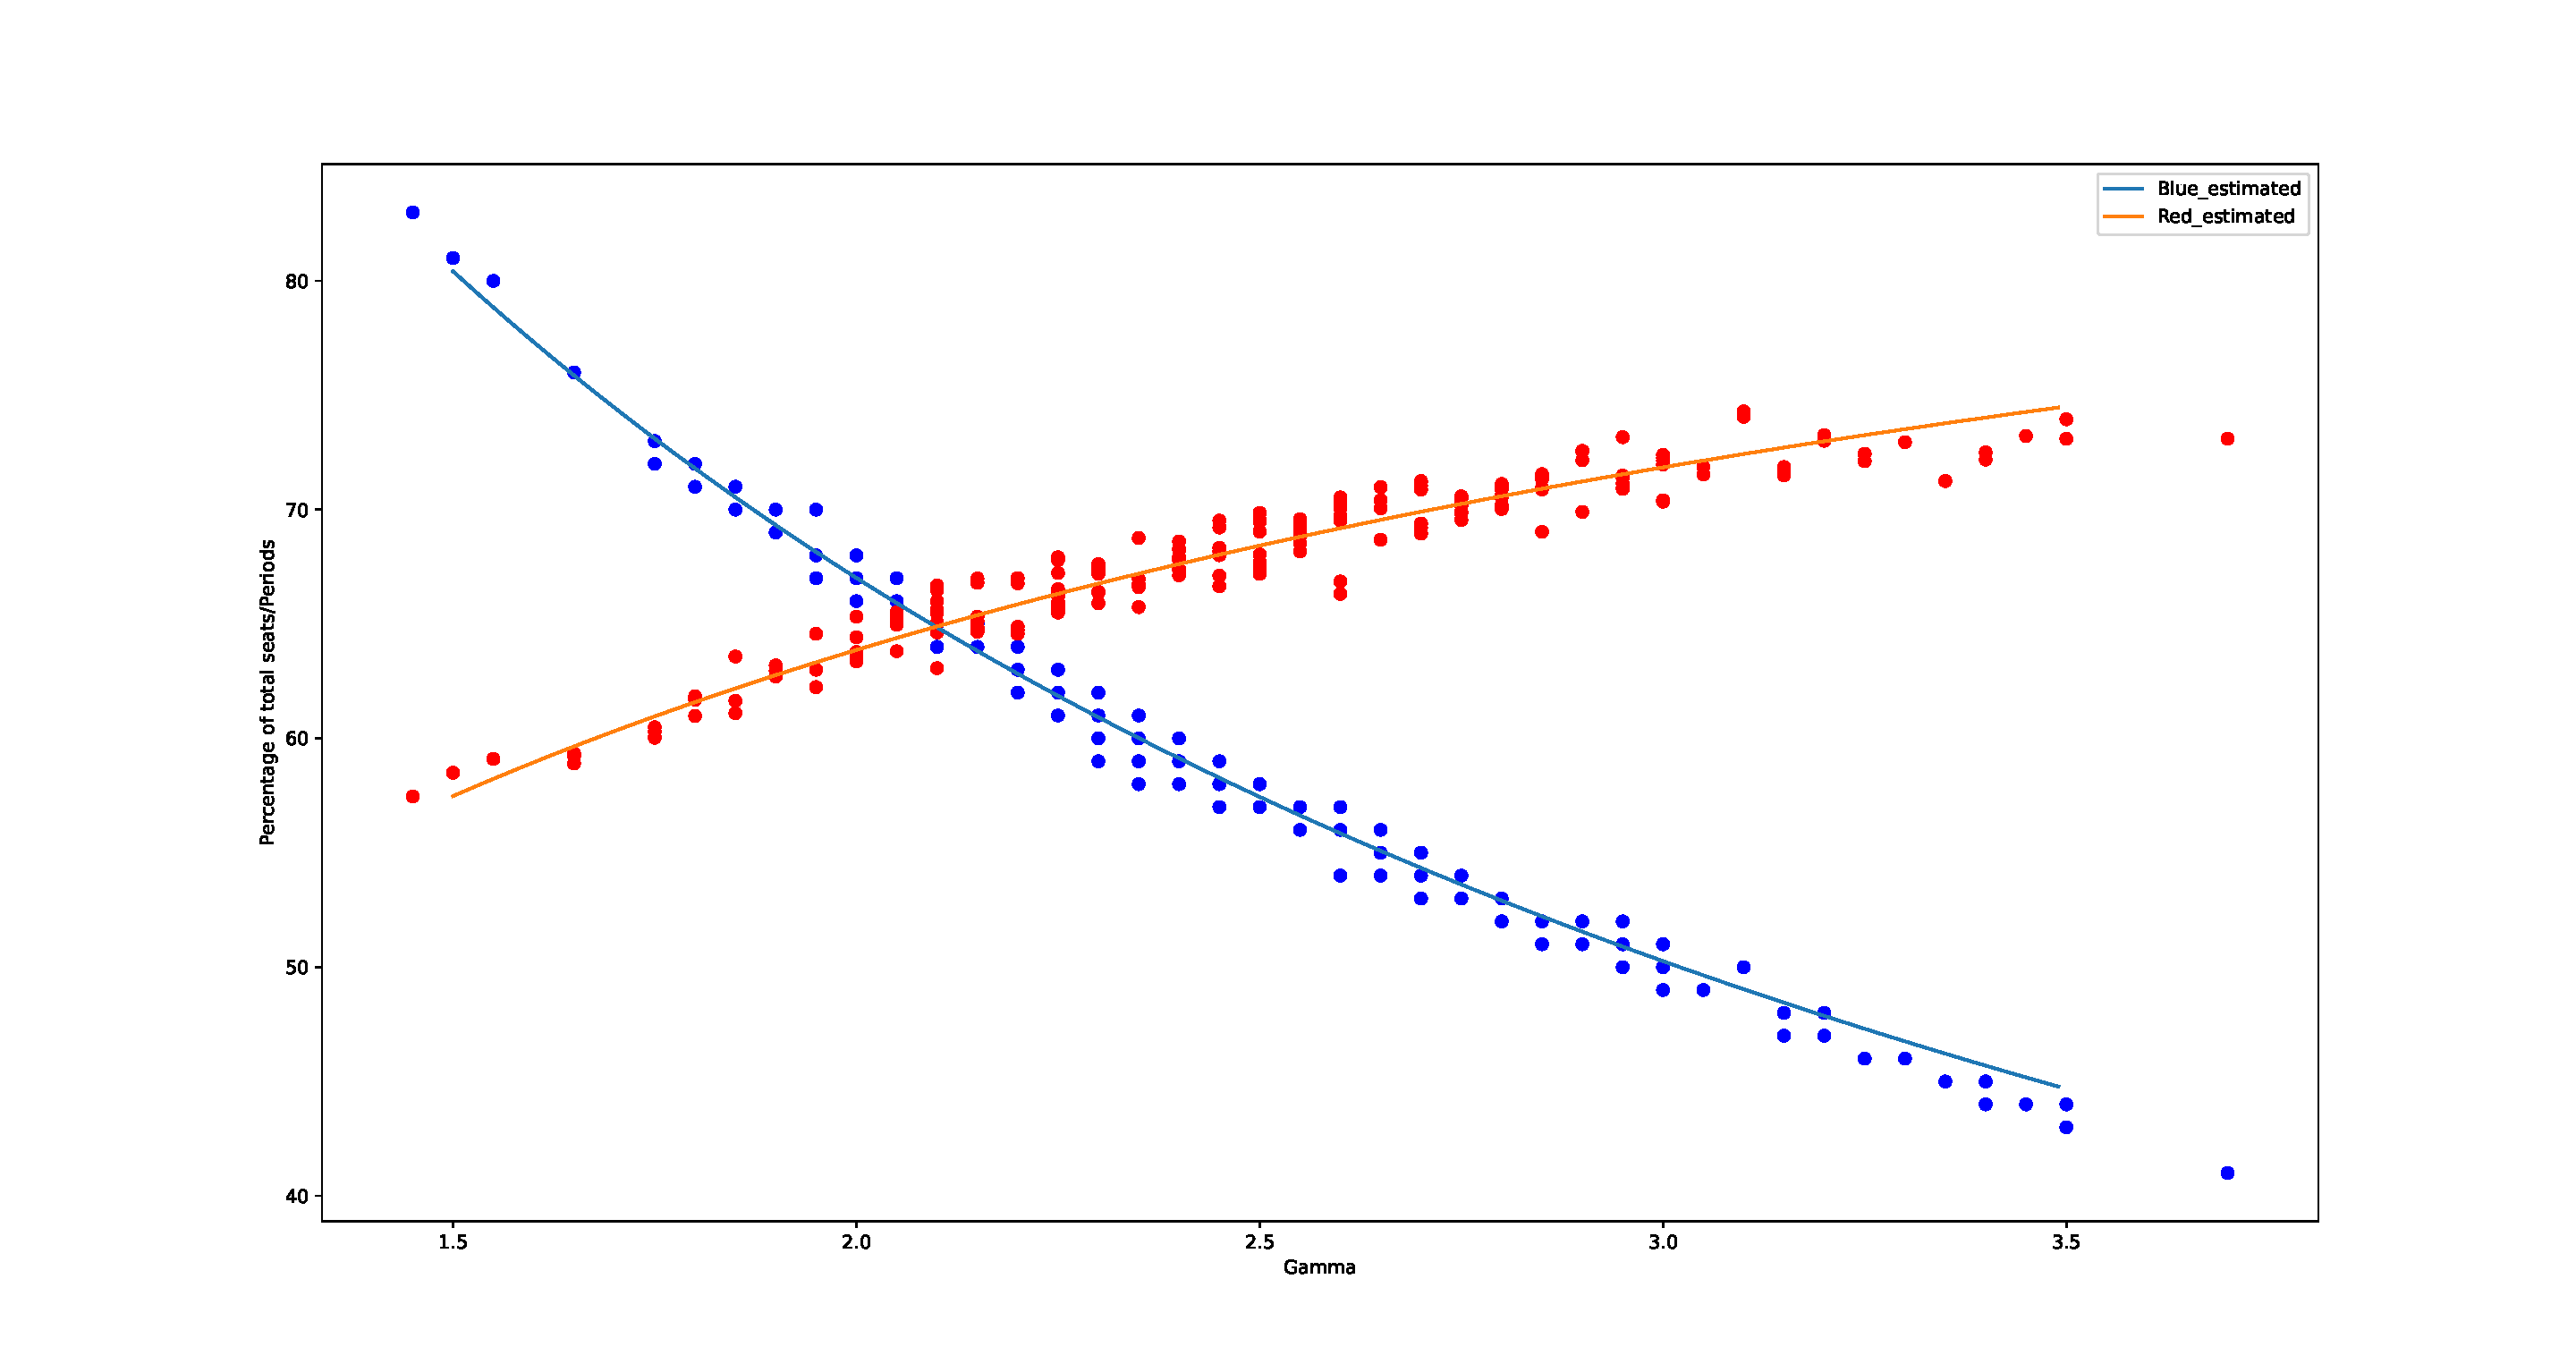
\includegraphics[width=0.8\textwidth]{./Figures/re2.pdf}
  \caption{Gap points and their estimation under 200 probabilities}
\end{figure}

The estimation of $c_1$ and $c_2$ can be affected by different seat layouts. To investigate this impact, we conduct several experiments using different seat layouts, specifically with the number of rows $\times$ the number of seats configurations set as 10 $\times$ 16, 10 $\times$ 21, 10 $\times$ 26 and 10 $\times$ 31. Similarly, we perform an analysis using a sample of 100 probability combinations, each with a mean equal to $\gamma$. The values of $\gamma$ range from 1.5 to 3.4. We employed an Ordinary Least Squares (OLS) model to fit the data and derive the parameter values. The goodness of fit is assessed using the R-square values, which are found to be 1.000 for all models, indicating a perfect fit between the data and the models.

The results of the estimation of $c_1$ and $c_2$ are presented in the table below:

\begin{table}[ht]
  \centering
  \caption{Estimation of $c_1$ and $c_2$}
  \begin{tabular}{|c|c|c|}
  \hline
   Seat layout(\# of rows $\times$ \# of seats) & Estimation of $c_1$ & Estimation of $c_2$  \\
  \hline
   10 $\times$ 11 & 0.909 $\pm$ 0.013  & 89.89 $\pm$ 1.436 \\
   10 $\times$ 16 & 0.948 $\pm$ 0.008  & 94.69 $\pm$ 0.802 \\
   10 $\times$ 21 & 0.955 $\pm$ 0.004 & 95.44 $\pm$ 0.571 \\
   10 $\times$ 26 & 0.966 $\pm$ 0.004 & 96.23 $\pm$ 0.386 \\
   10 $\times$ 31 & 0.965 $\pm$ 0.003 & 96.67 $\pm$ 0.434 \\
   10 $\times$ 36 & 0.968 $\pm$ 0.003 & 97.04 $\pm$ 0.289 \\
   \hline
  \end{tabular}
\end{table}


\subsubsection{Impact of Social Distancing as Demands Increase}
Now, we consider impact of social distance as demands increase by changing $T$. Specifically, we consider two situations: $\gamma = 1.9$ and $\gamma = 2.5$. We set the parameters as follows: $T$ varies from 30 to 120, the step size is 1.  The seat layout consists 10 rows and the number of seats per row is 21. The social distancing is 1 seat.

The figure below displays the outcomes of groups who were accepted under two different conditions: with social distancing measures and without social distancing measures. For the former case, we employ DSA to obtain the results. In this case, we consider the constraints of social distancing and optimize the seat allocation accordingly. For the latter case, we adopt a different approach. We simply accept all incoming groups as long as the capacity allows, without considering the constraints of groups needing to sit together. This means that we prioritize filling the available seats without enforcing any specific seating arrangements or social distancing requirements. We conduct an analysis using a sample of 100 probability combinations associated with the same $\gamma$. The occupancy rate at different demands is calculated as the mean of these 100 samples. The figures depicting the results are presented below.


\begin{figure}[h]
  \centering
  \subfigure[When $\gamma =1.9$]{
    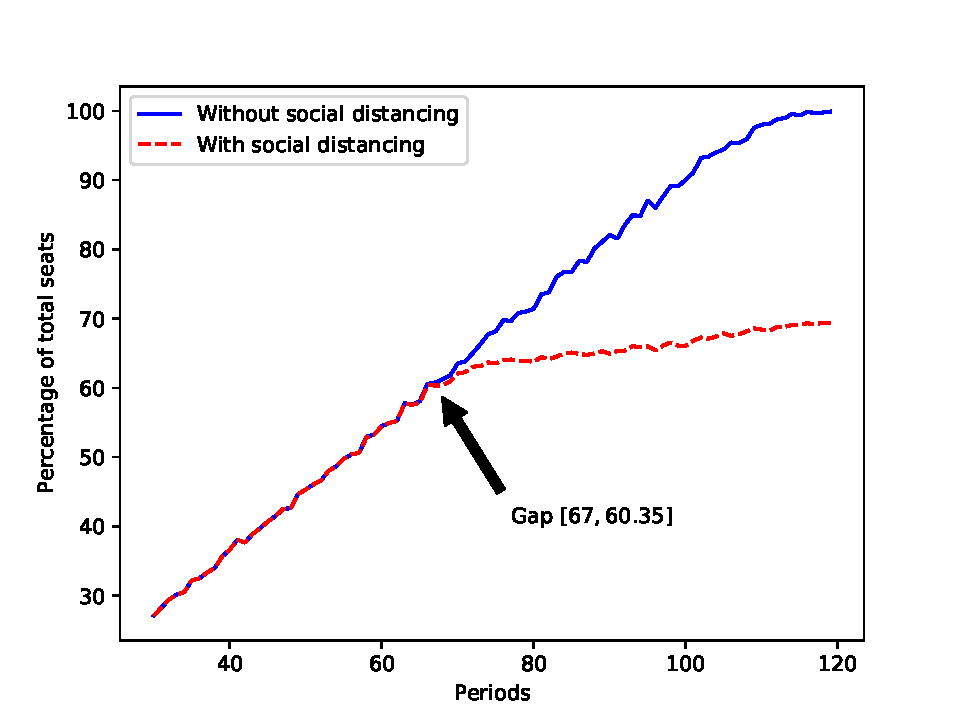
\includegraphics[width=0.48\textwidth]{./Figures/p2.pdf}}
  \subfigure[When $\gamma =2.5$]{
    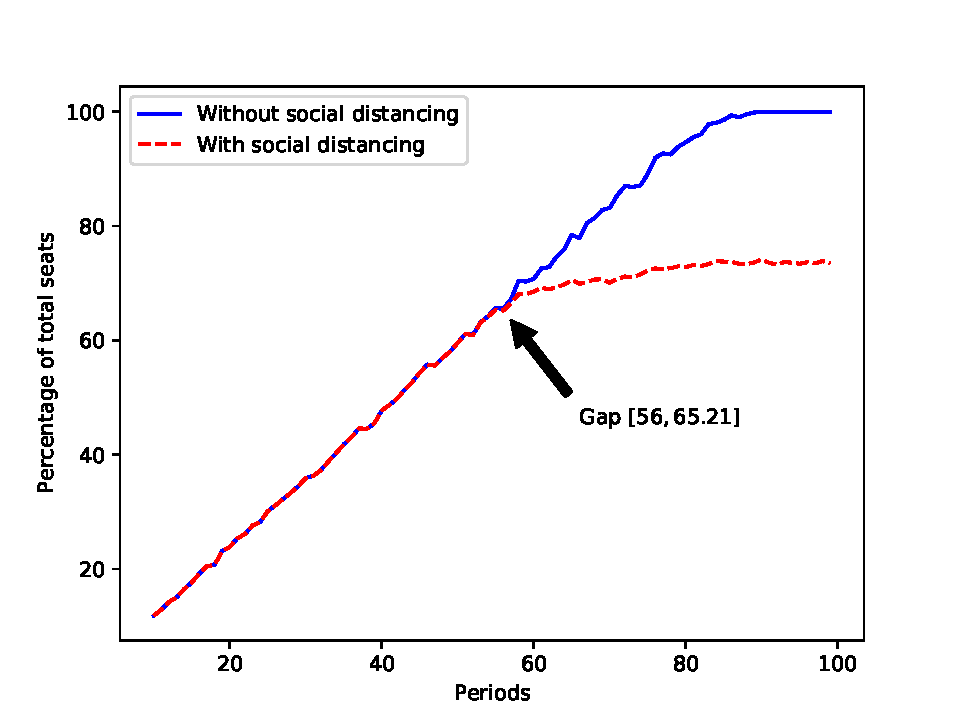
\includegraphics[width=0.48\textwidth]{./Figures/p1.pdf}}
  \caption{The occupancy rate over the number of arriving people}
\end{figure}

The analysis consists of three stages. 
In the first stage, when the capacity is sufficient, the outcome remains unaffected by the implementation of social distancing measures. In the second stage, as the value of $T$ increases, the difference between the outcomes with and without social distancing measures becomes more pronounced. Finally, in the third stage, as $T$ continues to increase, both scenarios reach their maximum capacity acceptance. At this point, the gap between the outcomes with and without social distancing measures begins to converge. For the social distancing situation, according to Proposition \ref{lem_pattern}, when the largest pattern is assigned to each row, the resulting occupancy rate is $\frac{16}{20} = 80\%$, which is the upper bound of occupancy rate.


The below table presents the percentage differences for different demand levels (130, 150, 170, 190, 210).



\begin{table}[ht]
  \centering
  \caption{Gap points and percentage differences under different demands of different gammas}
\begin{tabular}{lllllll}
  \hline
  \multicolumn{1}{|l|}{\multirow{2}{*}{$\gamma$}} & \multicolumn{1}{l|}{\multirow{2}{*}{gap point}} & \multicolumn{5}{l|}{percentage differences under different demands}   \\ 
  \cline{3-7} 
  \multicolumn{1}{|l|}{}                      & \multicolumn{1}{l|}{}                    & \multicolumn{1}{l|}{130} & \multicolumn{1}{l|}{150} & \multicolumn{1}{l|}{170} & \multicolumn{1}{l|}{190} & \multicolumn{1}{l|}{210} \\ 
  \hline
  \multicolumn{1}{|l|}{1.9}  & \multicolumn{1}{l|}{[69, 65.52]}  & \multicolumn{1}{l|}{0.25}  & \multicolumn{1}{l|}{5.82}  & \multicolumn{1}{l|}{12.82} & \multicolumn{1}{l|}{20.38} & \multicolumn{1}{l|}{24.56} \\ 
  \hline                                    
  \multicolumn{1}{|l|}{2.1}  & \multicolumn{1}{l|}{[64, 67.74]}  & \multicolumn{1}{l|}{0.05}  & \multicolumn{1}{l|}{4.11}  & \multicolumn{1}{l|}{11.51} & \multicolumn{1}{l|}{18.77} & \multicolumn{1}{l|}{21.87} \\ 
  \hline           
  \multicolumn{1}{|l|}{2.3}  & \multicolumn{1}{l|}{[61, 69.79]}  & \multicolumn{1}{l|}{0}  & \multicolumn{1}{l|}{2.29}  & \multicolumn{1}{l|}{10.21} & \multicolumn{1}{l|}{17.36} & \multicolumn{1}{l|}{21.16} \\ 
  \hline           
  \multicolumn{1}{|l|}{2.5}  & \multicolumn{1}{l|}{[57, 70.89]}  & \multicolumn{1}{l|}{0}  & \multicolumn{1}{l|}{1.45}  & \multicolumn{1}{l|}{9.30} & \multicolumn{1}{l|}{15.78} & \multicolumn{1}{l|}{19.80} \\ 
  \hline          
  \multicolumn{1}{|l|}{2.7}  & \multicolumn{1}{l|}{[53, 71.28]}  & \multicolumn{1}{l|}{0}  & \multicolumn{1}{l|}{1.38}  & \multicolumn{1}{l|}{7.39} & \multicolumn{1}{l|}{14.91} & \multicolumn{1}{l|}{19.14} \\ 
  \hline            
\end{tabular}
\end{table}



\subsection{Make the instant decision but late allocation}
We utilized bid-price control and dynamic programming in conducting the numerical experiments.

\begin{algorithm}[H]
  \caption{Bid-price Control Algorithm with Late Allocation}\label{algo_bid_late}
  \For{$t =1, \ldots, T$}{
    {Observe group type $i$\;}
    {Solve the LP relaxation of problem \eqref{deter_upper} with $d_i^{t} = (T-t) \cdot p_i$ and $\mathbf{L}^{t}$\;
    Obtain $\tilde{i}$ such that the aggregate optimal solution is $x e_{\tilde{i}} + \sum_{i=\tilde{i}+1} ^{M} d_{i} e_{i}$\;}
    \eIf{$i \geq \tilde{i}$ and }
    {Accept the group \;
    $\mathbf{L}^{t+1} \gets \mathbf{L}^{t} - n_i \mathbf{e}_{k}$\;}
    {Reject the group\; $\mathbf{L}^{t+1} \gets \mathbf{L}^{t}$\;}}
\end{algorithm}


\begin{table}[ht]
  \centering
  \begin{tabular}{|l|l|l|l|l|l|}
  \hline
   T & Probabilities &  DP1-L (\%) & Bid-L (\%) & DP1 (\%) & Bid (\%) \\
  \hline
  60  & [0.25, 0.25, 0.25, 0.25]  & 99.52 & 99.44 & 98.42 & 98.38 \\
  70  &   & 99.32 & 98.97 & 96.87 & 96.24 \\
  80  &   & 99.34 & 99.30 & 95.69 & 96.02 \\
  90  &   & 99.55 & 99.49 & 96.05 & 96.41  \\
  100 &   & 99.78 & 99.66 & 95.09 & 96.88 \\
  \hline
  60  & [0.25, 0.35, 0.05, 0.35]  & 99.50 & 99.37 & 98.26 & 98.25  \\
  70  &   & 99.40 & 98.97 & 96.62 & 96.06 \\
  80  &   & 99.46 & 99.24 & 96.01 & 95.89 \\
  90  &   & 99.59 & 99.35 & 96.77 & 96.62 \\
  100 &   & 99.77 & 99.61 & 97.04 & 97.14  \\
  \hline
  60  & [0.15, 0.25, 0.55, 0.05]  & 99.57 & 99.54 & 98.72 & 98.74 \\
  70  &   & 99.46 & 99.39  & 96.38 & 96.90 \\
  80  &   & 99.50 & 99.30  & 97.75 & 97.87 \\
  90  &   & 99.34 & 99.44  & 98.45 & 98.69 \\
  100 &   & 99.34 & 99.55  & 98.62 & 98.94 \\
  \hline
  \end{tabular}
\end{table}
% customer perference  选择


\newpage


